
% What is LATEX ?: LATEX is a tool used to create professional looking documents. LATEX principle - you focus on the content and let the computer manage the formatting of the document.
% What is the LATEX ADVANTAGE ?: It allows users to very quickly tackle the more complicated parts of type-setting such as inputting mathematics, tables, contents, references, etc. 
% One of the most important reasons people use LATEX is that it keeps the content and structure of your document cleanly separated from the formatting and allows for easy reuse as well as edit. Similarly, you can create one style of document which can be used to standardise the appearance of many different documents as a template.

% FIRST: comes the PREAMBLE of the Document.
% In the preamble you define the type of document you are writing, the language you are writing in, the packages you would like to use and several other elements.

\documentclass[12pt, letterpaper, twoside]{article} 
% The first line of code declares the type of the document, known as the CLASS. The class controls the overall appearance of the document, different types of documents will require different classes for instance; CV, Scientific Paper and more. 
% Some additional parameters included in the square brackets brackets, separated by commas can be passed to the command. In this case, the class is "article". The simplest and most common LATEX class and the extra parameters set the font size (12pt), paper size (letter paper). 
% "twoside" - In a two-sided document the space in the inner side of the page is a bit larger to help print and bind the book later on in a normal twosided manner. There are several commands that have a special version for two-sided documents, like figure alignment and page numbering

\usepackage[utf8]{inputenc} 
% This is the encoding for the document. It can be omitted or changed to another encoding but utf-8 is recommended.

% Adding a Title, Author and Date. 
\title{First Document and Tutorial\thanks{Thanks to the overleaf team.}}
\author{Aviral Janveja}
\date{\today}
% To add a title, author and date to our document, you must add above three lines to the preamble as shown. 
% The "thanks" command can be added inside the braces of the title command and is useful if you want to thank an institution in your article. It adds a superscript and a footnote.
% You can enter the date manually or use the command \today so the date will be updated automatically every time you compile your document.

% \usepackage{parskip} This is the recommended approach for adding  larger spaces between paragraphs. Instead of using multiple 'newline' commands. See the Paragraph and Newline section. 
\usepackage{graphicx}
% Latex can not manage images by itself, so we add the graphicx package to our preamble. Packages are used to change the default look of your document or to allow more functionalities and commands.
\graphicspath{{images/}}
% This command tells LATEX that the images are kept in a folder names 'images' under the current directory. 

% Everything in your .tex(LATEX) file before this point was the PREAMBLE.
% After this, you write the CONTENT of our DOCUMENT, enclosed inside the \begin{document} and \end{document} tags. This is known as the BODY of the document. 
\begin{document} 

\maketitle 
% The \maketitle command prints the title, author and date that you gave to your document in the preamble. This should be included in the body of your document at the place you want the title to be printed. (At the very top, for instance.)

\tableofcontents
% This command adds the table of contents to your document. See the table of contents section at the last. 

We have now added a title, author and date to our first \LaTeX{} document!

% COMMENT - by now you would have figured out that this how we add a comment to our LATEX code.

% BOLD, ITALICS, UNDERLINE & EMPHASIZE commands.
\textit{Italics}
\textbf{Bold}
\underline{Underline}.

Hi, This is an \emph{emphasize} example.

\textit{Hi, This is another \emph{emphasize} example.}

\textbf{Hi, This is yet another \emph{emphasize} example.}
% \emph emphasizes the chosen word differently depending on the current sentence formatting as displayed above.  


%Adding an IMAGE.
As you can see below on page \pageref{pic1}, In figure \ref{pic1}, Sadhguru talks about love.
\begin{figure}[t]
    \centering
    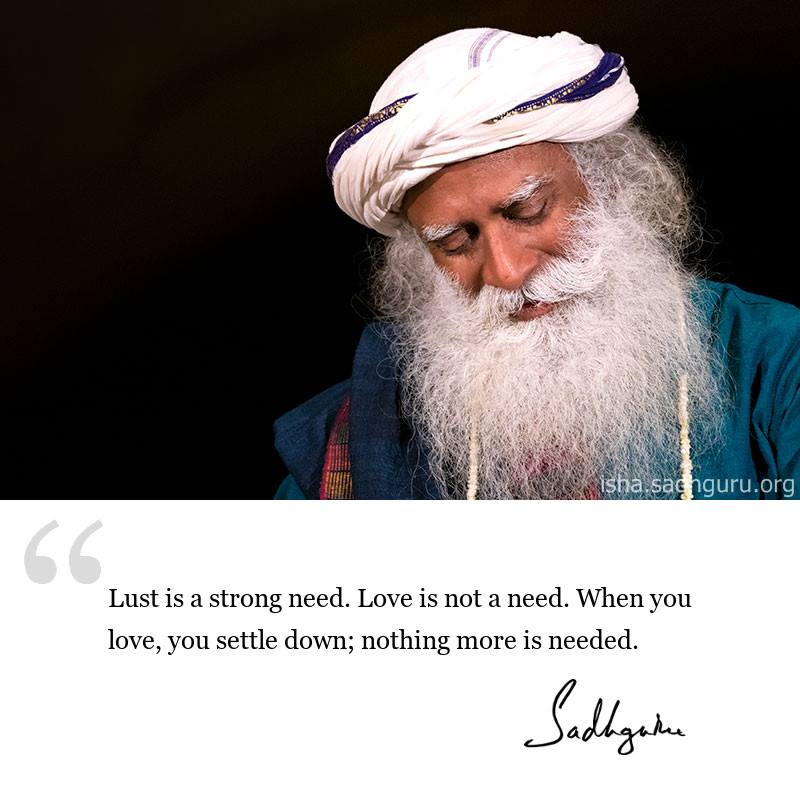
\includegraphics[width=0.25\textwidth]{love}
    \caption{Sadhguru on Love and Lust.}
    \label{pic1}
\end{figure}
% As shown above, Images can be CAPTIONED, LABELLED and REFERENCED by the means of the 'figure' environment. When placing images in a LATEX document, we should always put them inside a figure environment or similar so that LATEX will position the image in a way that fits in with the rest of your text.
% ENVIRONMENTS are sections of our document that you want to present in a different way to the rest of the document. They start with a \begin{...} command and end with an \end{...} command. Everything inside those commands will be formatted in a special manner depending on the type of the environment.
% \includegraphics{...} command is the one that actually included the IMAGE in the document. Here universe is the name of the file containing the image without the extension.
%  \caption{...} command sets the CAPTION for the figure. If you create a list of figures, this caption will be used there.
% \label{...} In case you need to refer to the image within your document.The label will number the image, and combined with the next command will allow you to reference it.
% \ref{...} This code will be substituted for by the number corresponding to the REFERENCED pic.

% Creating Lists in LATEX
% There are two main different types of lists, ordered lists and unordered lists. Each will use a different environment.

\begin{itemize}
    \item The unordered list using bullet-points.
    \item The text in the entries may be of any length. 
\end{itemize}
%Unordered lists are produced by the 'itemize' environment. Each entry must be preceded by the control sequence \item as shown below.

\begin{enumerate}
    \item The first entry starts at one. 
    \item The list numbers increase with each new entry.
\end{enumerate}
% Ordered list have the same syntax inside a different environment called 'enumerate'.


%Adding MATHEMATICS to Latex.
%LATEX allows two writing modes for mathematical expressions: the 'inline mode' and the 'display mode'.

In Physics, the mass-energy equivalence is stated by the equation \begin{math}E=mc^2\end{math} discovered in 1905 by Albert Einstein.
% The above is an inline mode example, used to write formulas that are part of a line or paragraph. To put your equations in inline mode use the delimiter: \begin{math} ... \end{math}.

The mass-energy equivalence is described by the famous equation
\begin{displaymath} E=mc^2 \end{displaymath} discovered by Albert Einstein in 1905.
% The display mode is used to write expressions that are not part of a line or paragraph, and are therefore put on separate lines.To print your equations in display mode use one of these delimiters: \begin{displaymath} ... \end{displaymath}.

%Many math mode commands require the amsmath package, so be sure to include it when writing math. An example is shown below of some basic math mode commands.
'Subscripts' in math mode are written as \begin{math}a_b\end{math} and 'superscripts' as \begin{math}a^b\end{math}.
These can be combined and nested to write expressions such as - 
\begin{displaymath}
T^{i_1i_2....i_p}_{j_1j_2...j_q} = T(x^{i_1},...,x^{i_p},e_{j_1},...,e_{j_q})
\end{displaymath}

We write integrals using \begin{math}\int\end{math} and fractions using \begin{math}\frac{a}{b}\end{math}. Limits are placed on integrals using superscripts and subscripts:
\begin{displaymath}
\int_0^1 \frac{1}{e^x} = \frac{e-1}{e}
\end{displaymath}
Lower case Greek letters are written as \begin{math}\omega\end{math}, \begin{math}\delta\end{math}, etc.
While upper case Greek letters are written as \begin{math}\Omega\end{math}, \begin{math}\Delta\end{math}.
Mathematical Operators are prefixed with a backslash as \begin{math}\sin(\beta),\cos(\alpha),\log(x)\end{math}, etc.

The possibilities with math in LATEX are endless and it is impossible to list them all here. Be sure to check out our other articles.


% BASIC FORMATTING.
We will now look at how to write abstracts, as well as how to format a Latex document into different chapters. 

% ABSTRACT
\begin{abstract}
In Scientific documents, it is a common practice to include a brief overview of the main subject of the paper. In Latex, there is the \textbf{abstract} environment for this. The abstract environment will put the text in a special format at the top of your document.     
\end{abstract}

% PARAGRAPHS AND NEWLINES
Now that we have written our abstract, we can begin writing our first paragraph. 

This line will start a second paragraph. \textbf{If you need to start a second paragraph, you must hit the enter key twice}. Notice that Latex automatically indents paragraphs. 

% To start a new line without actually starting a new paragraph insert a 'break line' point, this can be done by \\ (a double backslash) or the \newline command.
Hello, This is 
\\ a new line demonstration. 
\newline Hope you liked it. Bye! 

% Care must be take than multiple \\ or \newline are not used to simulate paragraphs with larger spacing between them. This can interfere with Latex's types-setting algorithms.
% The recommended approach is to use double blank lines only and then adding \usepackage{parskip} to the preamble.

% CHAPTERS AND SECTIONS - 
Commands to organize a document vary depending on the document type, the simplest form of organization is sectioning, available in all formats. 

%\part{} ;Only available in 'report' & 'book' document classes.

%\chapter{First Chapter} ;Only available in 'report' & 'book' document classes.

\section{Introduction} 
This is the first section.

In my first section, I would like to tell you that today I will be finishing with my Latex tutorial finally and starting to work on many documents and most importantly my CV in \LaTeX.

\section{Second Section}
This is the second section, I would like to tell you that today I will be finishing with my Latex tutorial finally and starting to work on many documents and most importantly my CV in \LaTeX.

\subsection{First Subsection}
In my first Subsection, I would like to tell you that today I will be finishing with my Latex tutorial finally and starting to work on many documents and most importantly my CV in \LaTeX.

\subsubsection{First Sub-subsection}
In my first Sub-subsection, I would like to tell you that today I will be finishing with my Latex tutorial finally and starting to work on many documents and most importantly my CV in \LaTeX.
\addcontentsline{toc}{section}{Unnumbered Section}
\section*{Unnumbered Section}
In my Unnumbered section, I would like to tell you that today I will be finishing with my Latex tutorial finally and starting to work on many documents and most importantly my CV in \LaTeX.
% The command \section{} marks the beginning of a new section, inside the braces is set the title. 
% Section numbering is automatic and can be disabled by including a * in the section command as \section*{}. 
% We can also have \subsection{}s, and indeed \subsubsection{}s. The basic levels of depth are listed below:
% \Part, \chapter, \section, \subsection, \subsubsection, \paragraph, \subparagraph.


CREATING TABLES - 
\begin{center}
\begin{tabular}{|c|c|c|}
\hline
cell1 & cell2 & cell3 \\
cell4 & cell5 & cell6 \\
cell7 & cell8 & cell9 \\
\hline
\end{tabular}    
\end{center}
% The tabular environment is the default LATEX method to create tables. You must specify a parameter to this environment, in this case {c c c}. This tells LATEX that there will be three columns and that the text inside each one of them must be centred. You can also use r to align the text to the right and l for left alignment.
%  The alignment symbol & is used to specify the breaks in the table entries. There must always be one less alignment symbol in each line than the number of columns.
% To go to the next line of your table, we use the new line command \\. We wrap the entire table inside the center environment so that it will appear in the center of the page.
% You can add borders using the horizontal line command \hline and the vertical line parameter '|'.
% {|c|c|c|}: This declares that three columns, separated by a vertical line, are going to be used in the table. The | symbol specifies that these columns should be separated by a vertical line.
% \hline: This will insert a horizontal line. We have included horizontal lines at the top and bottom of the table here. There is no restriction on the number of times you can use \hline.


A Second Example - with Captions, Labels \& References.
% Note how & is written with a forward slash as writing it normally produces an error.

% You can caption and reference tables in much the same way as images. The only difference is that instead of the figure environment, you use the table environment.
Table \ref{table1} is an example of referenced \LaTeX elements.
    \begin{table}[h!]
    \centering
    \begin{tabular}{||c|c|c|c||}
    \hline
    col1 & col2 & col3 & col4 \\[0.5ex]
    \hline\hline
    1 & 2 & 3 & 4 \\
    5 & 6 & 7 & 8 \\
    9 & 10 & 11 & 12 \\
    13 & 14 & 15 & 16 \\[0.5ex]
    \hline
    \end{tabular}
    \caption{Table to test Captions, Labels and Referencing.}
    \label{table1}
    \end{table}


% Adding a TABLE OF CONTENTS - 
% To create the table of contents is straightforward, the command \tableofcontents does all the work for you.
% Sections, subsections and chapters are automatically included in the table of contents. To manually add entries, for example when you want an unnumbered section, use the command \addcontentsline as shown in the 'Chapters and Sections' part of this document.

\textbf{As of this moment the \LaTeX tutorial is now complete. It is time to get your hands dirty. From now on, whenever you get stuck or need some additional guidance while working on \LaTeX, you can either revisit this document or visit the specific section of the overleaf documentation that addresses your problem. Have Fun!}

\textbf{The End.}
\end{document}